% Options for packages loaded elsewhere
\PassOptionsToPackage{unicode}{hyperref}
\PassOptionsToPackage{hyphens}{url}
\PassOptionsToPackage{dvipsnames,svgnames,x11names}{xcolor}
%
\documentclass[
  letterpaper,
  DIV=11,
  numbers=noendperiod]{scrartcl}

\usepackage{amsmath,amssymb}
\usepackage{iftex}
\ifPDFTeX
  \usepackage[T1]{fontenc}
  \usepackage[utf8]{inputenc}
  \usepackage{textcomp} % provide euro and other symbols
\else % if luatex or xetex
  \usepackage{unicode-math}
  \defaultfontfeatures{Scale=MatchLowercase}
  \defaultfontfeatures[\rmfamily]{Ligatures=TeX,Scale=1}
\fi
\usepackage{lmodern}
\ifPDFTeX\else  
    % xetex/luatex font selection
\fi
% Use upquote if available, for straight quotes in verbatim environments
\IfFileExists{upquote.sty}{\usepackage{upquote}}{}
\IfFileExists{microtype.sty}{% use microtype if available
  \usepackage[]{microtype}
  \UseMicrotypeSet[protrusion]{basicmath} % disable protrusion for tt fonts
}{}
\makeatletter
\@ifundefined{KOMAClassName}{% if non-KOMA class
  \IfFileExists{parskip.sty}{%
    \usepackage{parskip}
  }{% else
    \setlength{\parindent}{0pt}
    \setlength{\parskip}{6pt plus 2pt minus 1pt}}
}{% if KOMA class
  \KOMAoptions{parskip=half}}
\makeatother
\usepackage{xcolor}
\setlength{\emergencystretch}{3em} % prevent overfull lines
\setcounter{secnumdepth}{5}
% Make \paragraph and \subparagraph free-standing
\ifx\paragraph\undefined\else
  \let\oldparagraph\paragraph
  \renewcommand{\paragraph}[1]{\oldparagraph{#1}\mbox{}}
\fi
\ifx\subparagraph\undefined\else
  \let\oldsubparagraph\subparagraph
  \renewcommand{\subparagraph}[1]{\oldsubparagraph{#1}\mbox{}}
\fi

\usepackage{color}
\usepackage{fancyvrb}
\newcommand{\VerbBar}{|}
\newcommand{\VERB}{\Verb[commandchars=\\\{\}]}
\DefineVerbatimEnvironment{Highlighting}{Verbatim}{commandchars=\\\{\}}
% Add ',fontsize=\small' for more characters per line
\usepackage{framed}
\definecolor{shadecolor}{RGB}{241,243,245}
\newenvironment{Shaded}{\begin{snugshade}}{\end{snugshade}}
\newcommand{\AlertTok}[1]{\textcolor[rgb]{0.68,0.00,0.00}{#1}}
\newcommand{\AnnotationTok}[1]{\textcolor[rgb]{0.37,0.37,0.37}{#1}}
\newcommand{\AttributeTok}[1]{\textcolor[rgb]{0.40,0.45,0.13}{#1}}
\newcommand{\BaseNTok}[1]{\textcolor[rgb]{0.68,0.00,0.00}{#1}}
\newcommand{\BuiltInTok}[1]{\textcolor[rgb]{0.00,0.23,0.31}{#1}}
\newcommand{\CharTok}[1]{\textcolor[rgb]{0.13,0.47,0.30}{#1}}
\newcommand{\CommentTok}[1]{\textcolor[rgb]{0.37,0.37,0.37}{#1}}
\newcommand{\CommentVarTok}[1]{\textcolor[rgb]{0.37,0.37,0.37}{\textit{#1}}}
\newcommand{\ConstantTok}[1]{\textcolor[rgb]{0.56,0.35,0.01}{#1}}
\newcommand{\ControlFlowTok}[1]{\textcolor[rgb]{0.00,0.23,0.31}{#1}}
\newcommand{\DataTypeTok}[1]{\textcolor[rgb]{0.68,0.00,0.00}{#1}}
\newcommand{\DecValTok}[1]{\textcolor[rgb]{0.68,0.00,0.00}{#1}}
\newcommand{\DocumentationTok}[1]{\textcolor[rgb]{0.37,0.37,0.37}{\textit{#1}}}
\newcommand{\ErrorTok}[1]{\textcolor[rgb]{0.68,0.00,0.00}{#1}}
\newcommand{\ExtensionTok}[1]{\textcolor[rgb]{0.00,0.23,0.31}{#1}}
\newcommand{\FloatTok}[1]{\textcolor[rgb]{0.68,0.00,0.00}{#1}}
\newcommand{\FunctionTok}[1]{\textcolor[rgb]{0.28,0.35,0.67}{#1}}
\newcommand{\ImportTok}[1]{\textcolor[rgb]{0.00,0.46,0.62}{#1}}
\newcommand{\InformationTok}[1]{\textcolor[rgb]{0.37,0.37,0.37}{#1}}
\newcommand{\KeywordTok}[1]{\textcolor[rgb]{0.00,0.23,0.31}{#1}}
\newcommand{\NormalTok}[1]{\textcolor[rgb]{0.00,0.23,0.31}{#1}}
\newcommand{\OperatorTok}[1]{\textcolor[rgb]{0.37,0.37,0.37}{#1}}
\newcommand{\OtherTok}[1]{\textcolor[rgb]{0.00,0.23,0.31}{#1}}
\newcommand{\PreprocessorTok}[1]{\textcolor[rgb]{0.68,0.00,0.00}{#1}}
\newcommand{\RegionMarkerTok}[1]{\textcolor[rgb]{0.00,0.23,0.31}{#1}}
\newcommand{\SpecialCharTok}[1]{\textcolor[rgb]{0.37,0.37,0.37}{#1}}
\newcommand{\SpecialStringTok}[1]{\textcolor[rgb]{0.13,0.47,0.30}{#1}}
\newcommand{\StringTok}[1]{\textcolor[rgb]{0.13,0.47,0.30}{#1}}
\newcommand{\VariableTok}[1]{\textcolor[rgb]{0.07,0.07,0.07}{#1}}
\newcommand{\VerbatimStringTok}[1]{\textcolor[rgb]{0.13,0.47,0.30}{#1}}
\newcommand{\WarningTok}[1]{\textcolor[rgb]{0.37,0.37,0.37}{\textit{#1}}}

\providecommand{\tightlist}{%
  \setlength{\itemsep}{0pt}\setlength{\parskip}{0pt}}\usepackage{longtable,booktabs,array}
\usepackage{calc} % for calculating minipage widths
% Correct order of tables after \paragraph or \subparagraph
\usepackage{etoolbox}
\makeatletter
\patchcmd\longtable{\par}{\if@noskipsec\mbox{}\fi\par}{}{}
\makeatother
% Allow footnotes in longtable head/foot
\IfFileExists{footnotehyper.sty}{\usepackage{footnotehyper}}{\usepackage{footnote}}
\makesavenoteenv{longtable}
\usepackage{graphicx}
\makeatletter
\def\maxwidth{\ifdim\Gin@nat@width>\linewidth\linewidth\else\Gin@nat@width\fi}
\def\maxheight{\ifdim\Gin@nat@height>\textheight\textheight\else\Gin@nat@height\fi}
\makeatother
% Scale images if necessary, so that they will not overflow the page
% margins by default, and it is still possible to overwrite the defaults
% using explicit options in \includegraphics[width, height, ...]{}
\setkeys{Gin}{width=\maxwidth,height=\maxheight,keepaspectratio}
% Set default figure placement to htbp
\makeatletter
\def\fps@figure{htbp}
\makeatother

\KOMAoption{captions}{tableheading}
\makeatletter
\@ifpackageloaded{caption}{}{\usepackage{caption}}
\AtBeginDocument{%
\ifdefined\contentsname
  \renewcommand*\contentsname{Table of contents}
\else
  \newcommand\contentsname{Table of contents}
\fi
\ifdefined\listfigurename
  \renewcommand*\listfigurename{List of Figures}
\else
  \newcommand\listfigurename{List of Figures}
\fi
\ifdefined\listtablename
  \renewcommand*\listtablename{List of Tables}
\else
  \newcommand\listtablename{List of Tables}
\fi
\ifdefined\figurename
  \renewcommand*\figurename{Figure}
\else
  \newcommand\figurename{Figure}
\fi
\ifdefined\tablename
  \renewcommand*\tablename{Table}
\else
  \newcommand\tablename{Table}
\fi
}
\@ifpackageloaded{float}{}{\usepackage{float}}
\floatstyle{ruled}
\@ifundefined{c@chapter}{\newfloat{codelisting}{h}{lop}}{\newfloat{codelisting}{h}{lop}[chapter]}
\floatname{codelisting}{Listing}
\newcommand*\listoflistings{\listof{codelisting}{List of Listings}}
\makeatother
\makeatletter
\makeatother
\makeatletter
\@ifpackageloaded{caption}{}{\usepackage{caption}}
\@ifpackageloaded{subcaption}{}{\usepackage{subcaption}}
\makeatother
\ifLuaTeX
  \usepackage{selnolig}  % disable illegal ligatures
\fi
\usepackage{bookmark}

\IfFileExists{xurl.sty}{\usepackage{xurl}}{} % add URL line breaks if available
\urlstyle{same} % disable monospaced font for URLs
\hypersetup{
  pdftitle={Data Visualization With Stata (The Basics)},
  pdfauthor={Andy Grogan-Kaylor},
  colorlinks=true,
  linkcolor={blue},
  filecolor={Maroon},
  citecolor={Blue},
  urlcolor={Blue},
  pdfcreator={LaTeX via pandoc}}

\title{Data Visualization With Stata (The Basics)}
\author{Andy Grogan-Kaylor}
\date{2024-05-13}

\begin{document}
\maketitle

\renewcommand*\contentsname{Table of contents}
{
\hypersetup{linkcolor=}
\setcounter{tocdepth}{3}
\tableofcontents
}
\section{Introduction}\label{introduction}

99\% of data visualization work seems to consist of creating bar graphs
(\texttt{graph\ bar\ y,\ over(x)}) and scatterplots
(\texttt{twoway\ scatter\ y\ x}). (For the sake of completeness, I am
also going to mention histograms (\texttt{histogram\ x}).)

\begin{quote}
Note: In some commands, I use \texttt{///} so that Stata commands can be
on multiple lines.
\end{quote}

This is a quick guide to these ideas using the
\href{https://github.com/allisonhorst/palmerpenguins/blob/master/README.md}{Palmer
Penguins Data}.

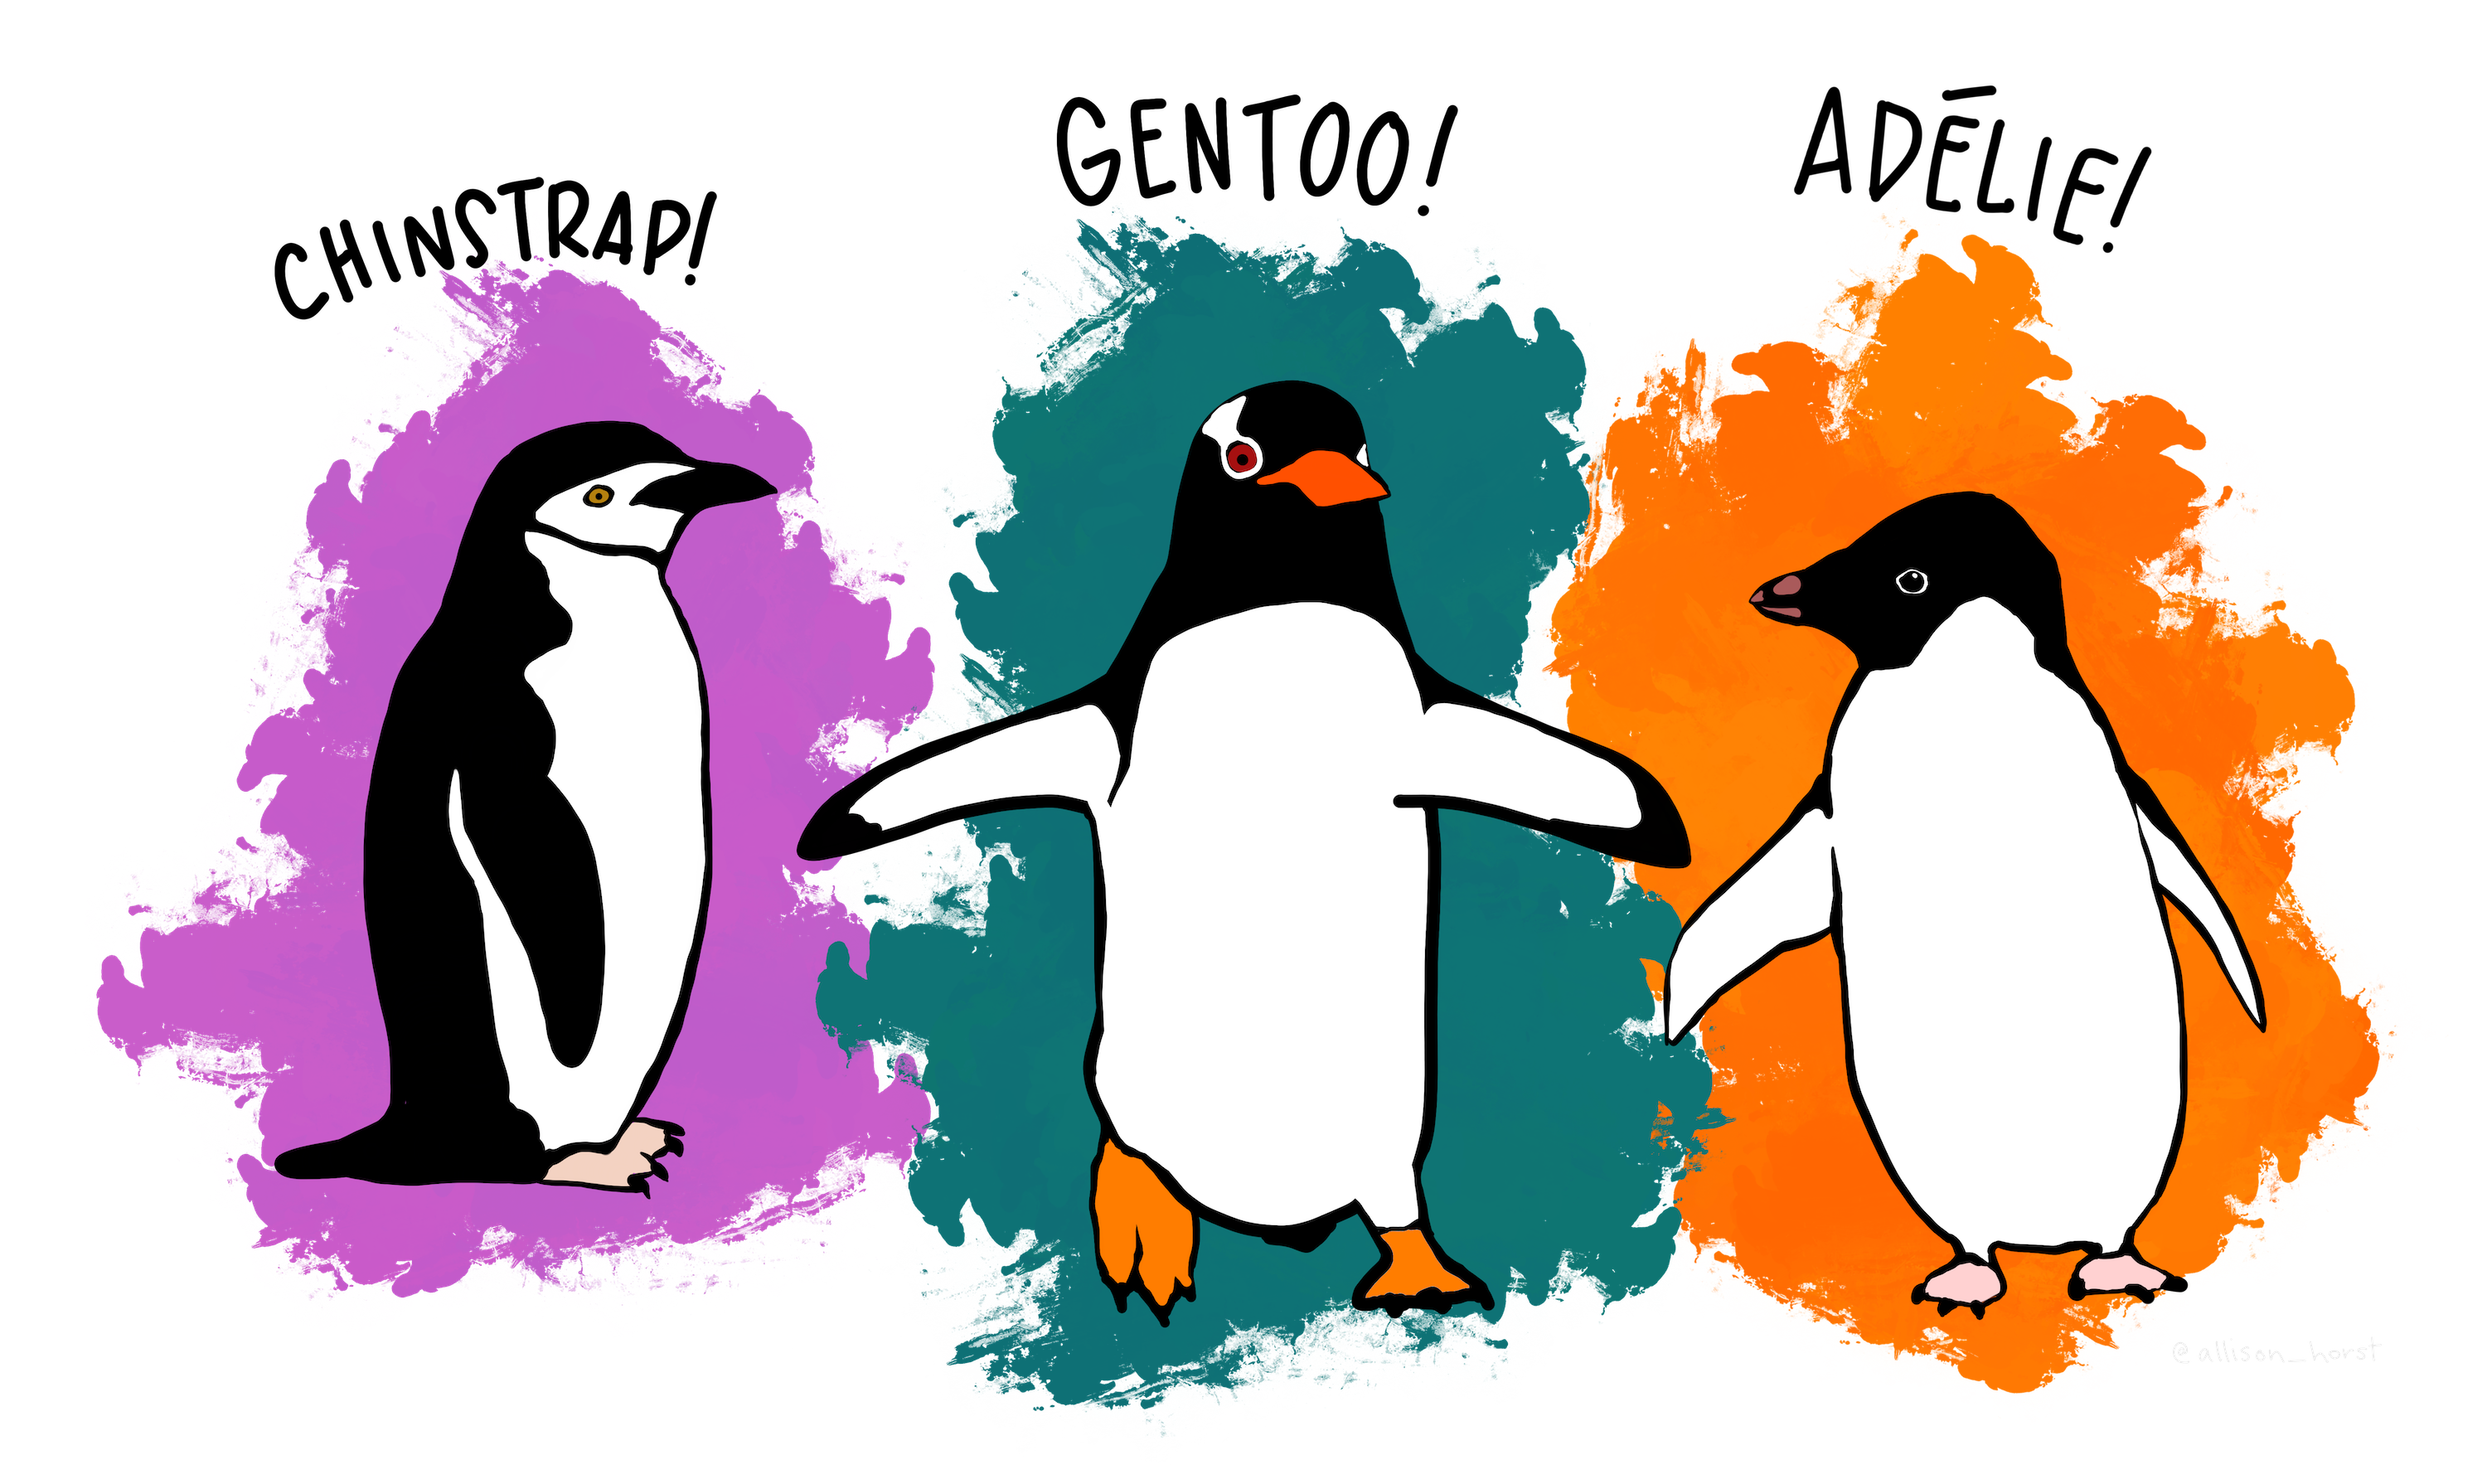
\includegraphics[width=0.2\textwidth,height=\textheight]{lter_penguins.png}
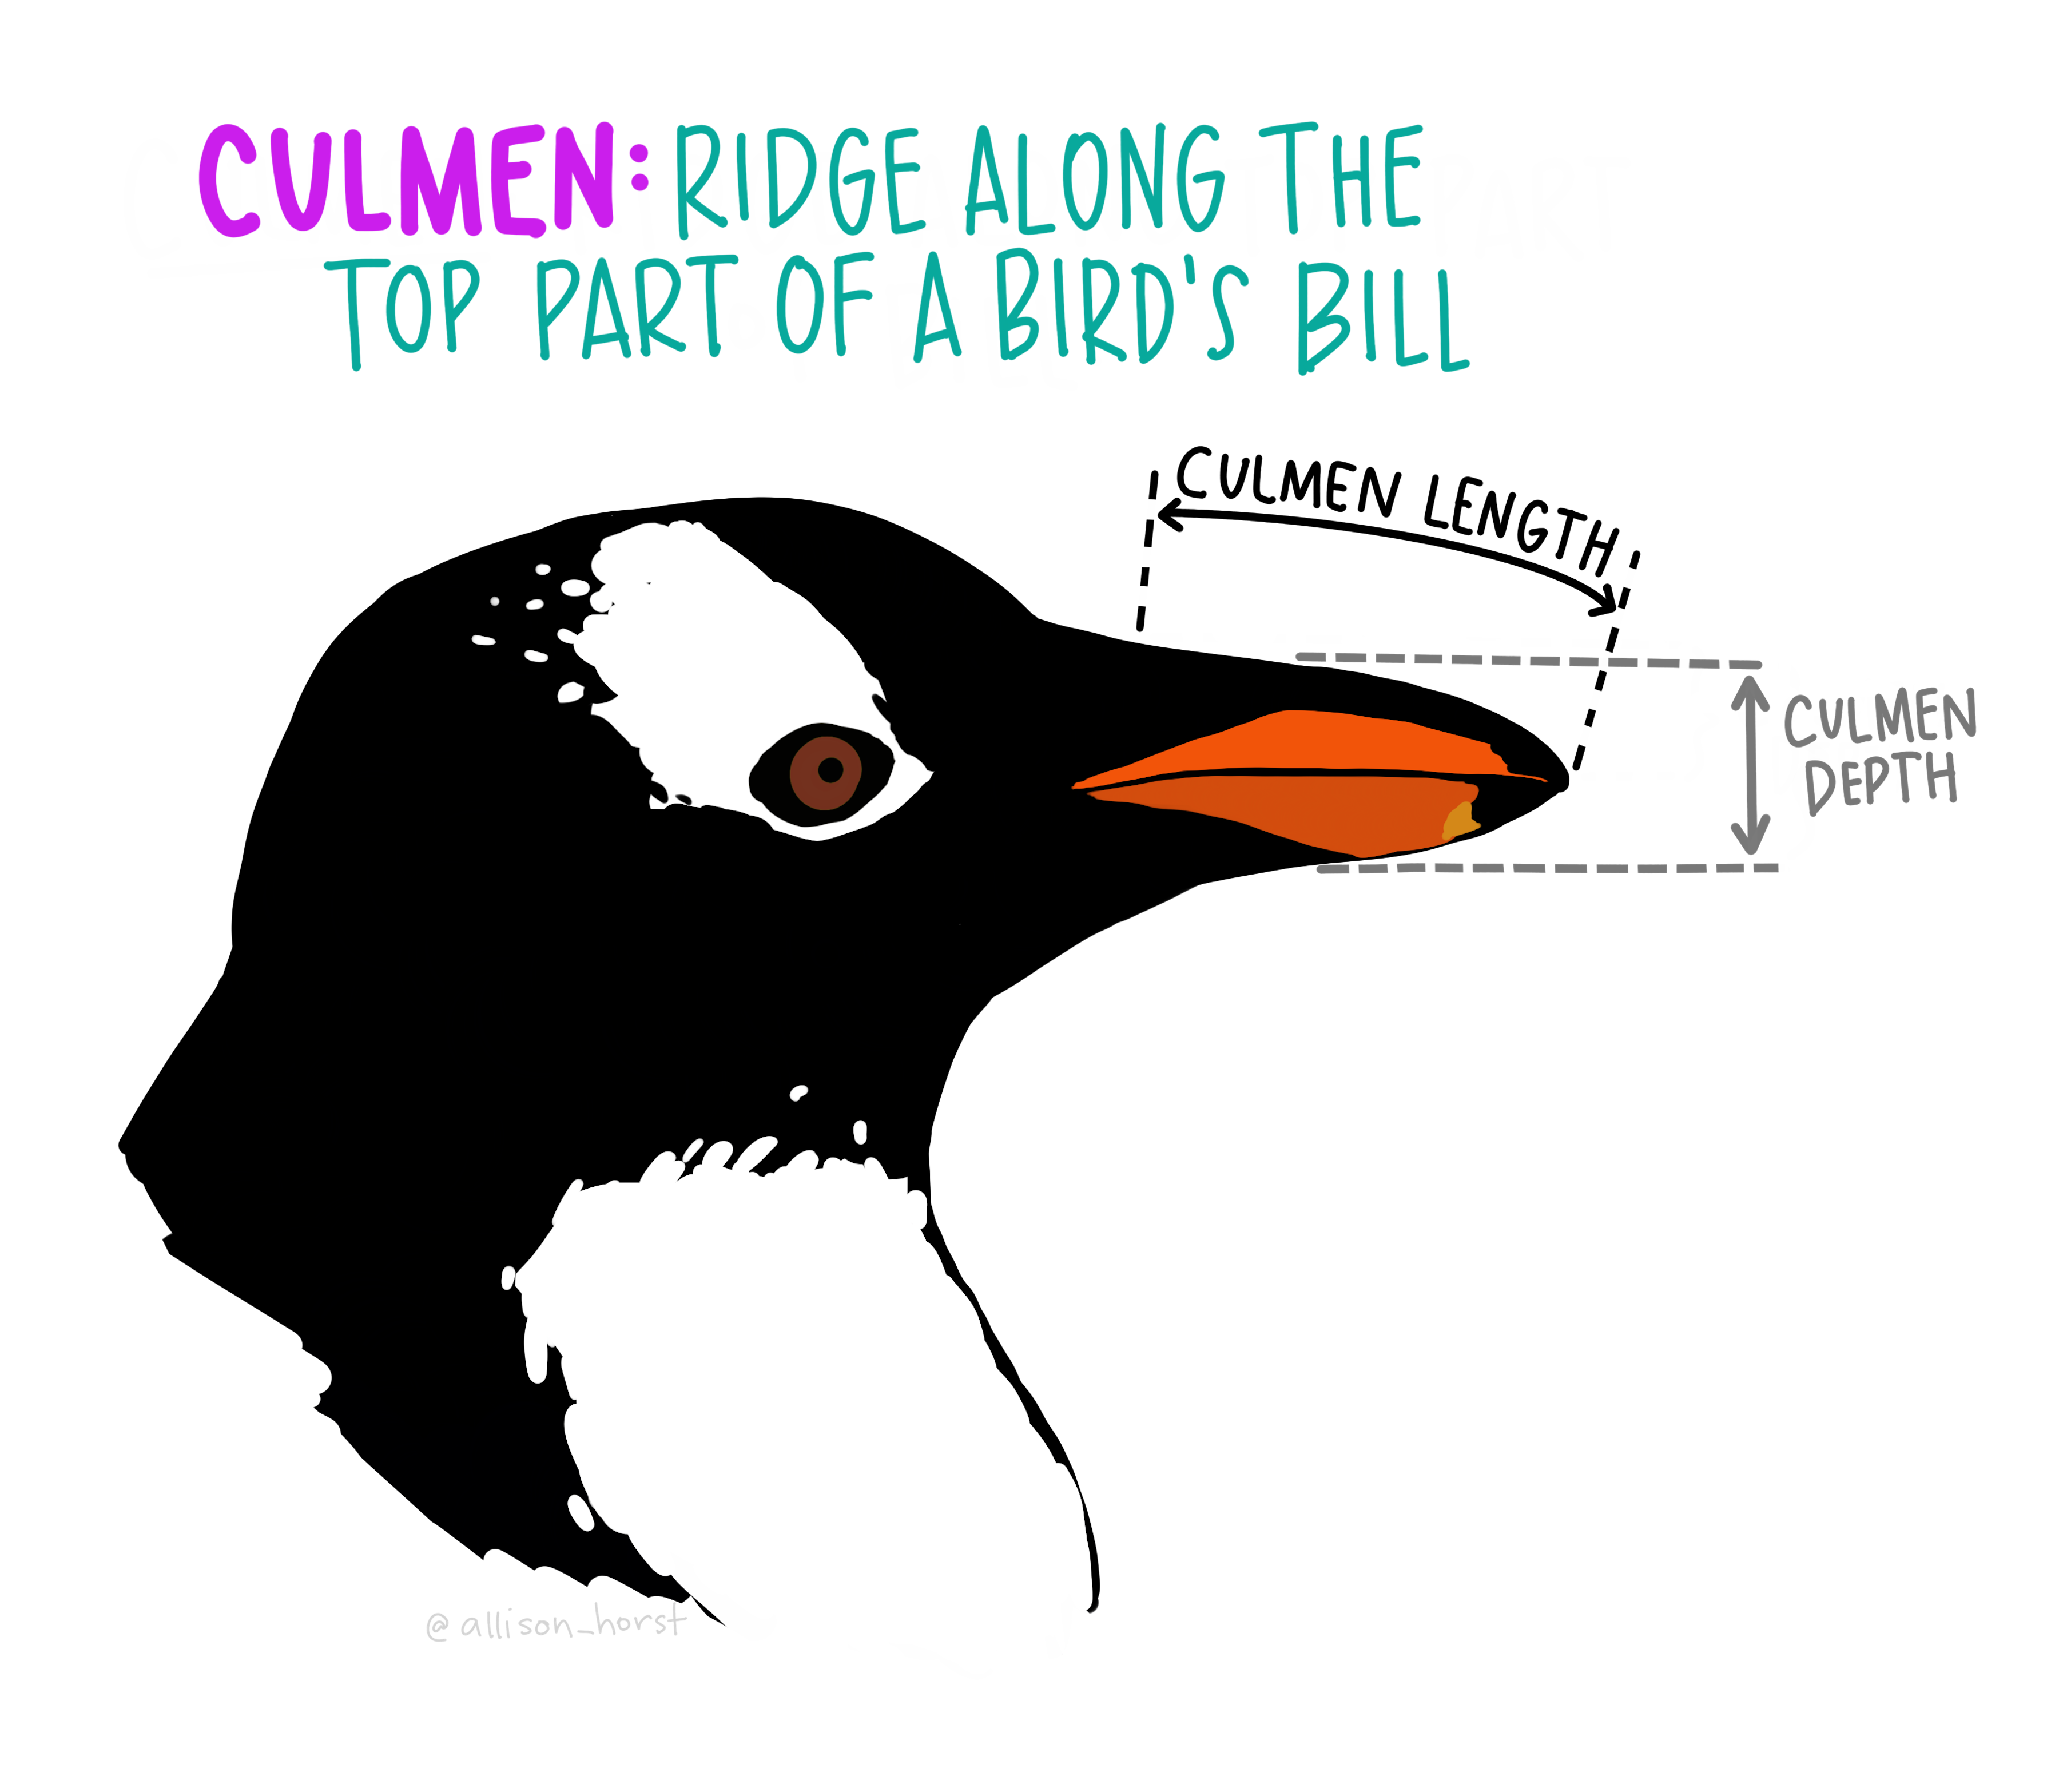
\includegraphics[width=0.2\textwidth,height=\textheight]{culmen_depth.png}

\section{Setup}\label{setup}

\begin{Shaded}
\begin{Highlighting}[]

\KeywordTok{clear} \OtherTok{all}

\KeywordTok{use} \StringTok{"penguins.dta"}\NormalTok{, }\KeywordTok{clear}
\end{Highlighting}
\end{Shaded}

Or, click
\href{https://github.com/agrogan1/Stata/raw/master/data-visualization-with-Stata-the-basics/penguins.dta}{here}
to download the data.

\begin{quote}
I am not a particular fan of the default \texttt{s2color} graph scheme
in earlier versions of Stata. In earlier versions of Stata, I might use
the \texttt{s1color} scheme by typing \texttt{set\ scheme\ s1color}.
This handout makes use of the \texttt{stcolor} graph scheme which is the
default in newer versions of Stata.
\end{quote}

\section{\texorpdfstring{Histogram:
\texttt{histogram\ x}}{Histogram: histogram x}}\label{histogram-histogram-x}

\begin{Shaded}
\begin{Highlighting}[]
\KeywordTok{histogram}\NormalTok{ body\_mass\_g, }\BaseNTok{title}\NormalTok{(}\StringTok{"Body Mass of Penguins"}\NormalTok{) }\BaseNTok{xtitle}\NormalTok{(}\StringTok{"Body Mass"}\NormalTok{)}
\end{Highlighting}
\end{Shaded}

\begin{figure}[H]

{\centering 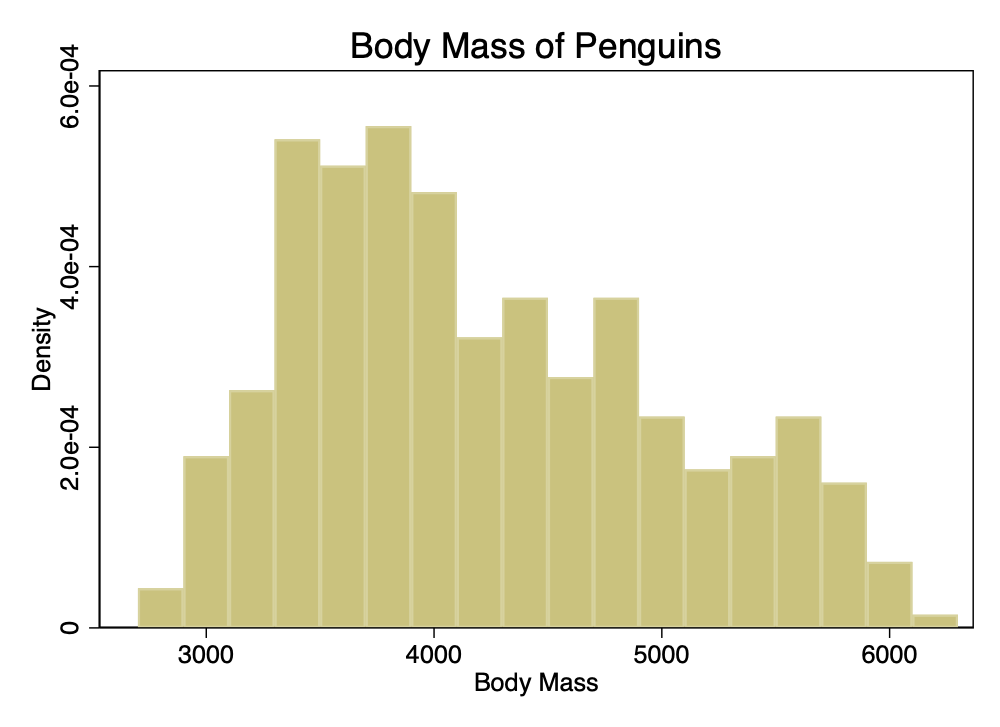
\includegraphics[width=0.25\textwidth,height=\textheight]{myhistogram.png}

}

\caption{histogram}

\end{figure}%

\section{\texorpdfstring{Bar Graph:
\texttt{graph\ bar}}{Bar Graph: graph bar}}\label{bar-graph-graph-bar}

\subsection{\texorpdfstring{Counting Up Numbers In Each Group:
\texttt{graph\ bar,\ over(x)}}{Counting Up Numbers In Each Group: graph bar, over(x)}}\label{counting-up-numbers-in-each-group-graph-bar-overx}

\begin{Shaded}
\begin{Highlighting}[]
\KeywordTok{graph} \BaseNTok{bar}\NormalTok{, }\BaseNTok{over}\NormalTok{(species) }\BaseNTok{title}\NormalTok{(}\StringTok{"Penguin Species"}\NormalTok{)}
\end{Highlighting}
\end{Shaded}

\begin{figure}[H]

{\centering 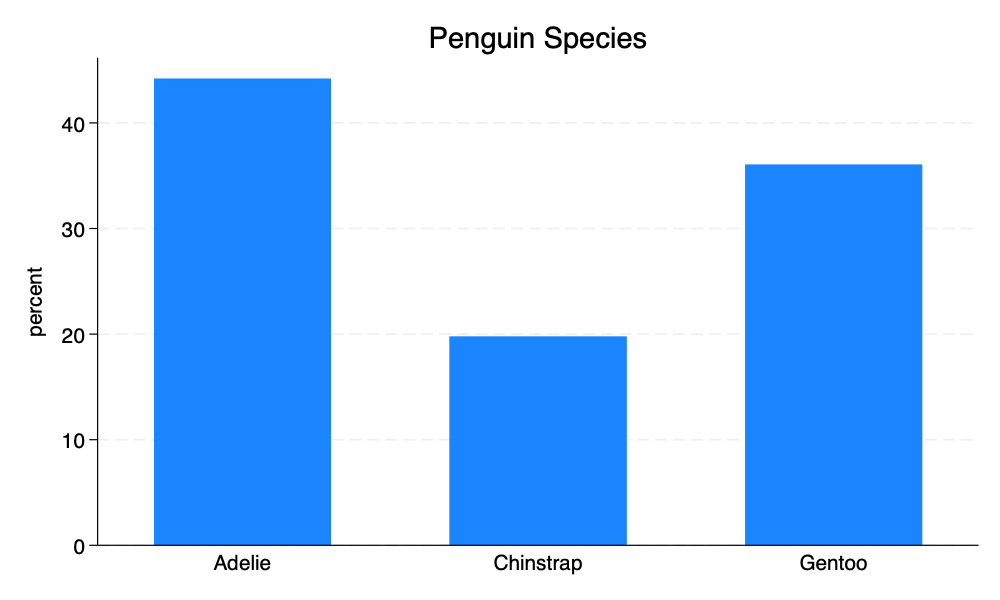
\includegraphics[width=0.3\textwidth,height=\textheight]{mybar1.png}

}

\caption{bar graph}

\end{figure}%

\subsection{\texorpdfstring{Average Of A Continuous Variable Across
Groups:
\texttt{graph\ bar\ y,\ over(x)}}{Average Of A Continuous Variable Across Groups: graph bar y, over(x)}}\label{average-of-a-continuous-variable-across-groups-graph-bar-y-overx}

\begin{Shaded}
\begin{Highlighting}[]
\KeywordTok{graph} \BaseNTok{bar}\NormalTok{ body\_mass\_g, }\BaseNTok{over}\NormalTok{(species) }\BaseNTok{title}\NormalTok{(}\StringTok{"Body Mass of Penguin Species"}\NormalTok{)}
\end{Highlighting}
\end{Shaded}

\begin{figure}[H]

{\centering 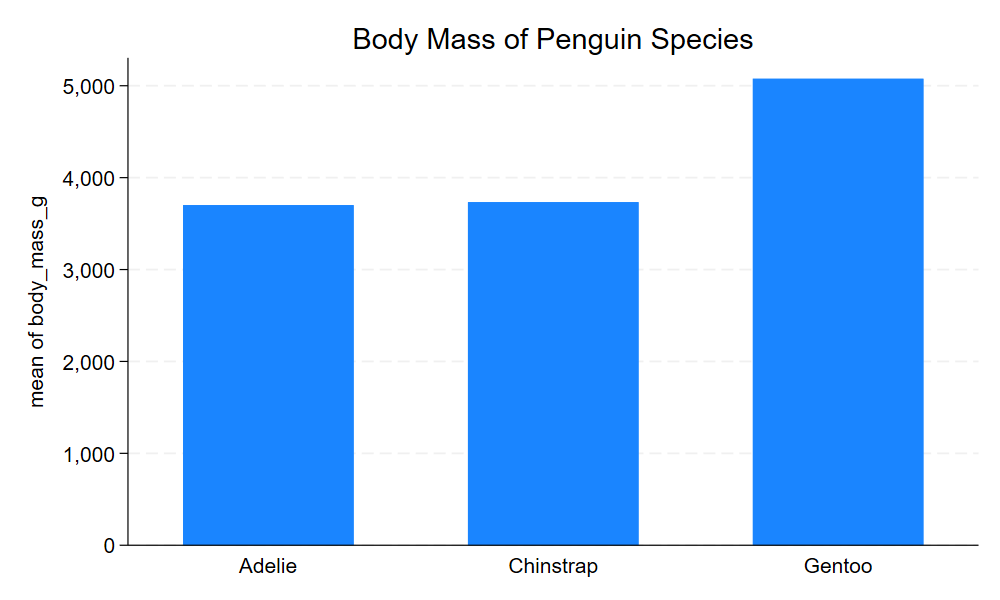
\includegraphics[width=0.3\textwidth,height=\textheight]{mybar2.png}

}

\caption{bar graph}

\end{figure}%

\section{\texorpdfstring{Scatterplot:
\texttt{twoway\ scatter\ y\ x}}{Scatterplot: twoway scatter y x}}\label{scatterplot-twoway-scatter-y-x}

\begin{Shaded}
\begin{Highlighting}[]
\KeywordTok{twoway} \KeywordTok{scatter}\NormalTok{ culmen\_length\_mm body\_mass\_g, }\CommentTok{///}
\BaseNTok{title}\NormalTok{(}\StringTok{"Penguin Culmen Length by Body Mass"}\NormalTok{) }\CommentTok{/// }
\BaseNTok{xtitle}\NormalTok{(}\StringTok{"Body Mass"}\NormalTok{) }\CommentTok{///}
\BaseNTok{ytitle}\NormalTok{(}\StringTok{"Culmen Length"}\NormalTok{)}
\end{Highlighting}
\end{Shaded}

\begin{figure}[H]

{\centering 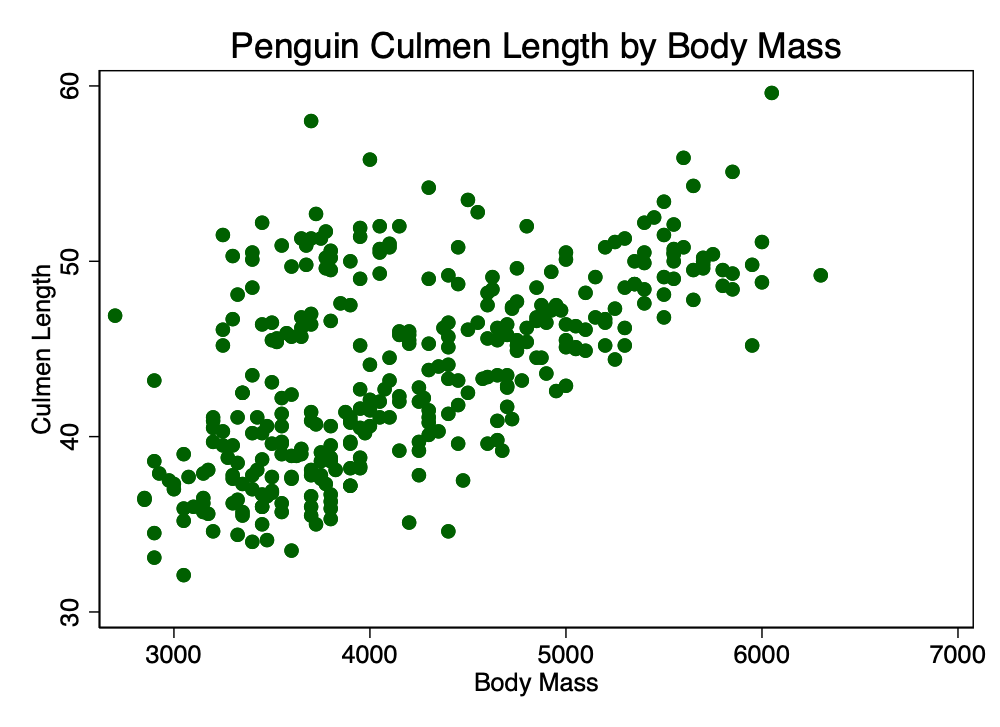
\includegraphics[width=0.3\textwidth,height=\textheight]{myscatter.png}

}

\caption{scatterplot}

\end{figure}%

\section{\texorpdfstring{Linear Fit:
\texttt{twoway\ lfit\ y\ x}}{Linear Fit: twoway lfit y x}}\label{linear-fit-twoway-lfit-y-x}

\begin{Shaded}
\begin{Highlighting}[]
\KeywordTok{twoway} \KeywordTok{lfit}\NormalTok{ culmen\_length\_mm body\_mass\_g, }\CommentTok{///}
\BaseNTok{title}\NormalTok{(}\StringTok{"Penguin Culmen Length by Body Mass"}\NormalTok{) }\CommentTok{/// }
\BaseNTok{xtitle}\NormalTok{(}\StringTok{"Body Mass"}\NormalTok{) }\CommentTok{///}
\BaseNTok{ytitle}\NormalTok{(}\StringTok{"Culmen Length"}\NormalTok{)}
\end{Highlighting}
\end{Shaded}

\begin{figure}[H]

{\centering 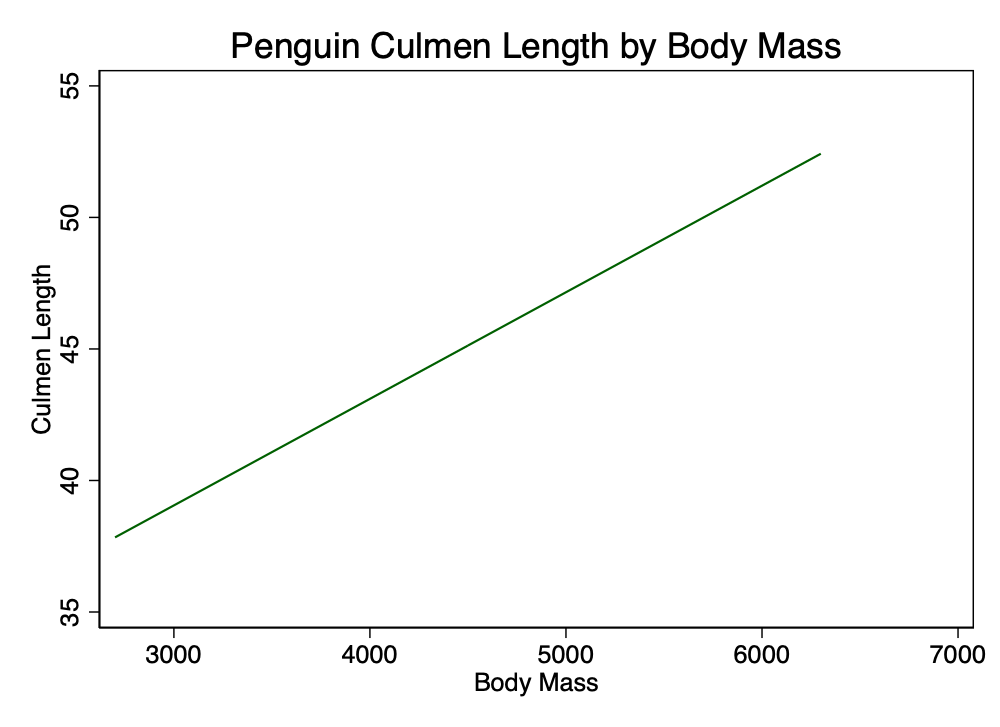
\includegraphics[width=0.3\textwidth,height=\textheight]{mylinear.png}

}

\caption{scatterplot}

\end{figure}%



\end{document}
